% ========================================================
% ------------ Appendix: More Visualization --------------
% ========================================================

\section{More Visualization}\label{sec:appendix_visualization}
\setnavsection{sec:appendix_visualization}

\renewcommand{\thefigure}{F\arabic{figure}}
\renewcommand{\theHfigure}{F\arabic{figure}}
\setcounter{figure}{0}

\renewcommand{\thetable}{F\arabic{table}}
\renewcommand{\theHtable}{F\arabic{table}}
\setcounter{table}{0}


\subsection{Cross-Benchmark Capability Analysis for Text Generation}\label{sec:appendix_benchmark}

As shown in \textbf{Section \ref{sec:evaluation_toL}}, we identify a set of generalized, high-level capability dimensions that transcend benchmark boundaries, namely state transition, commonsense reasoning, spatial relations, and dynamic motion.
Several representative examples are provided below.

\begin{figure}[!htbp]
    \centering
    \includegraphics[width=0.94\linewidth]{figs/appendix/state-1.pdf}
    \caption{\textbf{Cross-benchmark examples of state transition.} This dimension evaluates a model’s understanding of causal temporal dynamics and physical state changes, namely its ability to predict or recognize the evolution of an object from state A to state B. The improvement is particularly evident in tasks involving irreversible physical processes.}
    \label{fig:state-cross-bench1}
\end{figure}

\begin{figure}[!htbp]
    \centering
    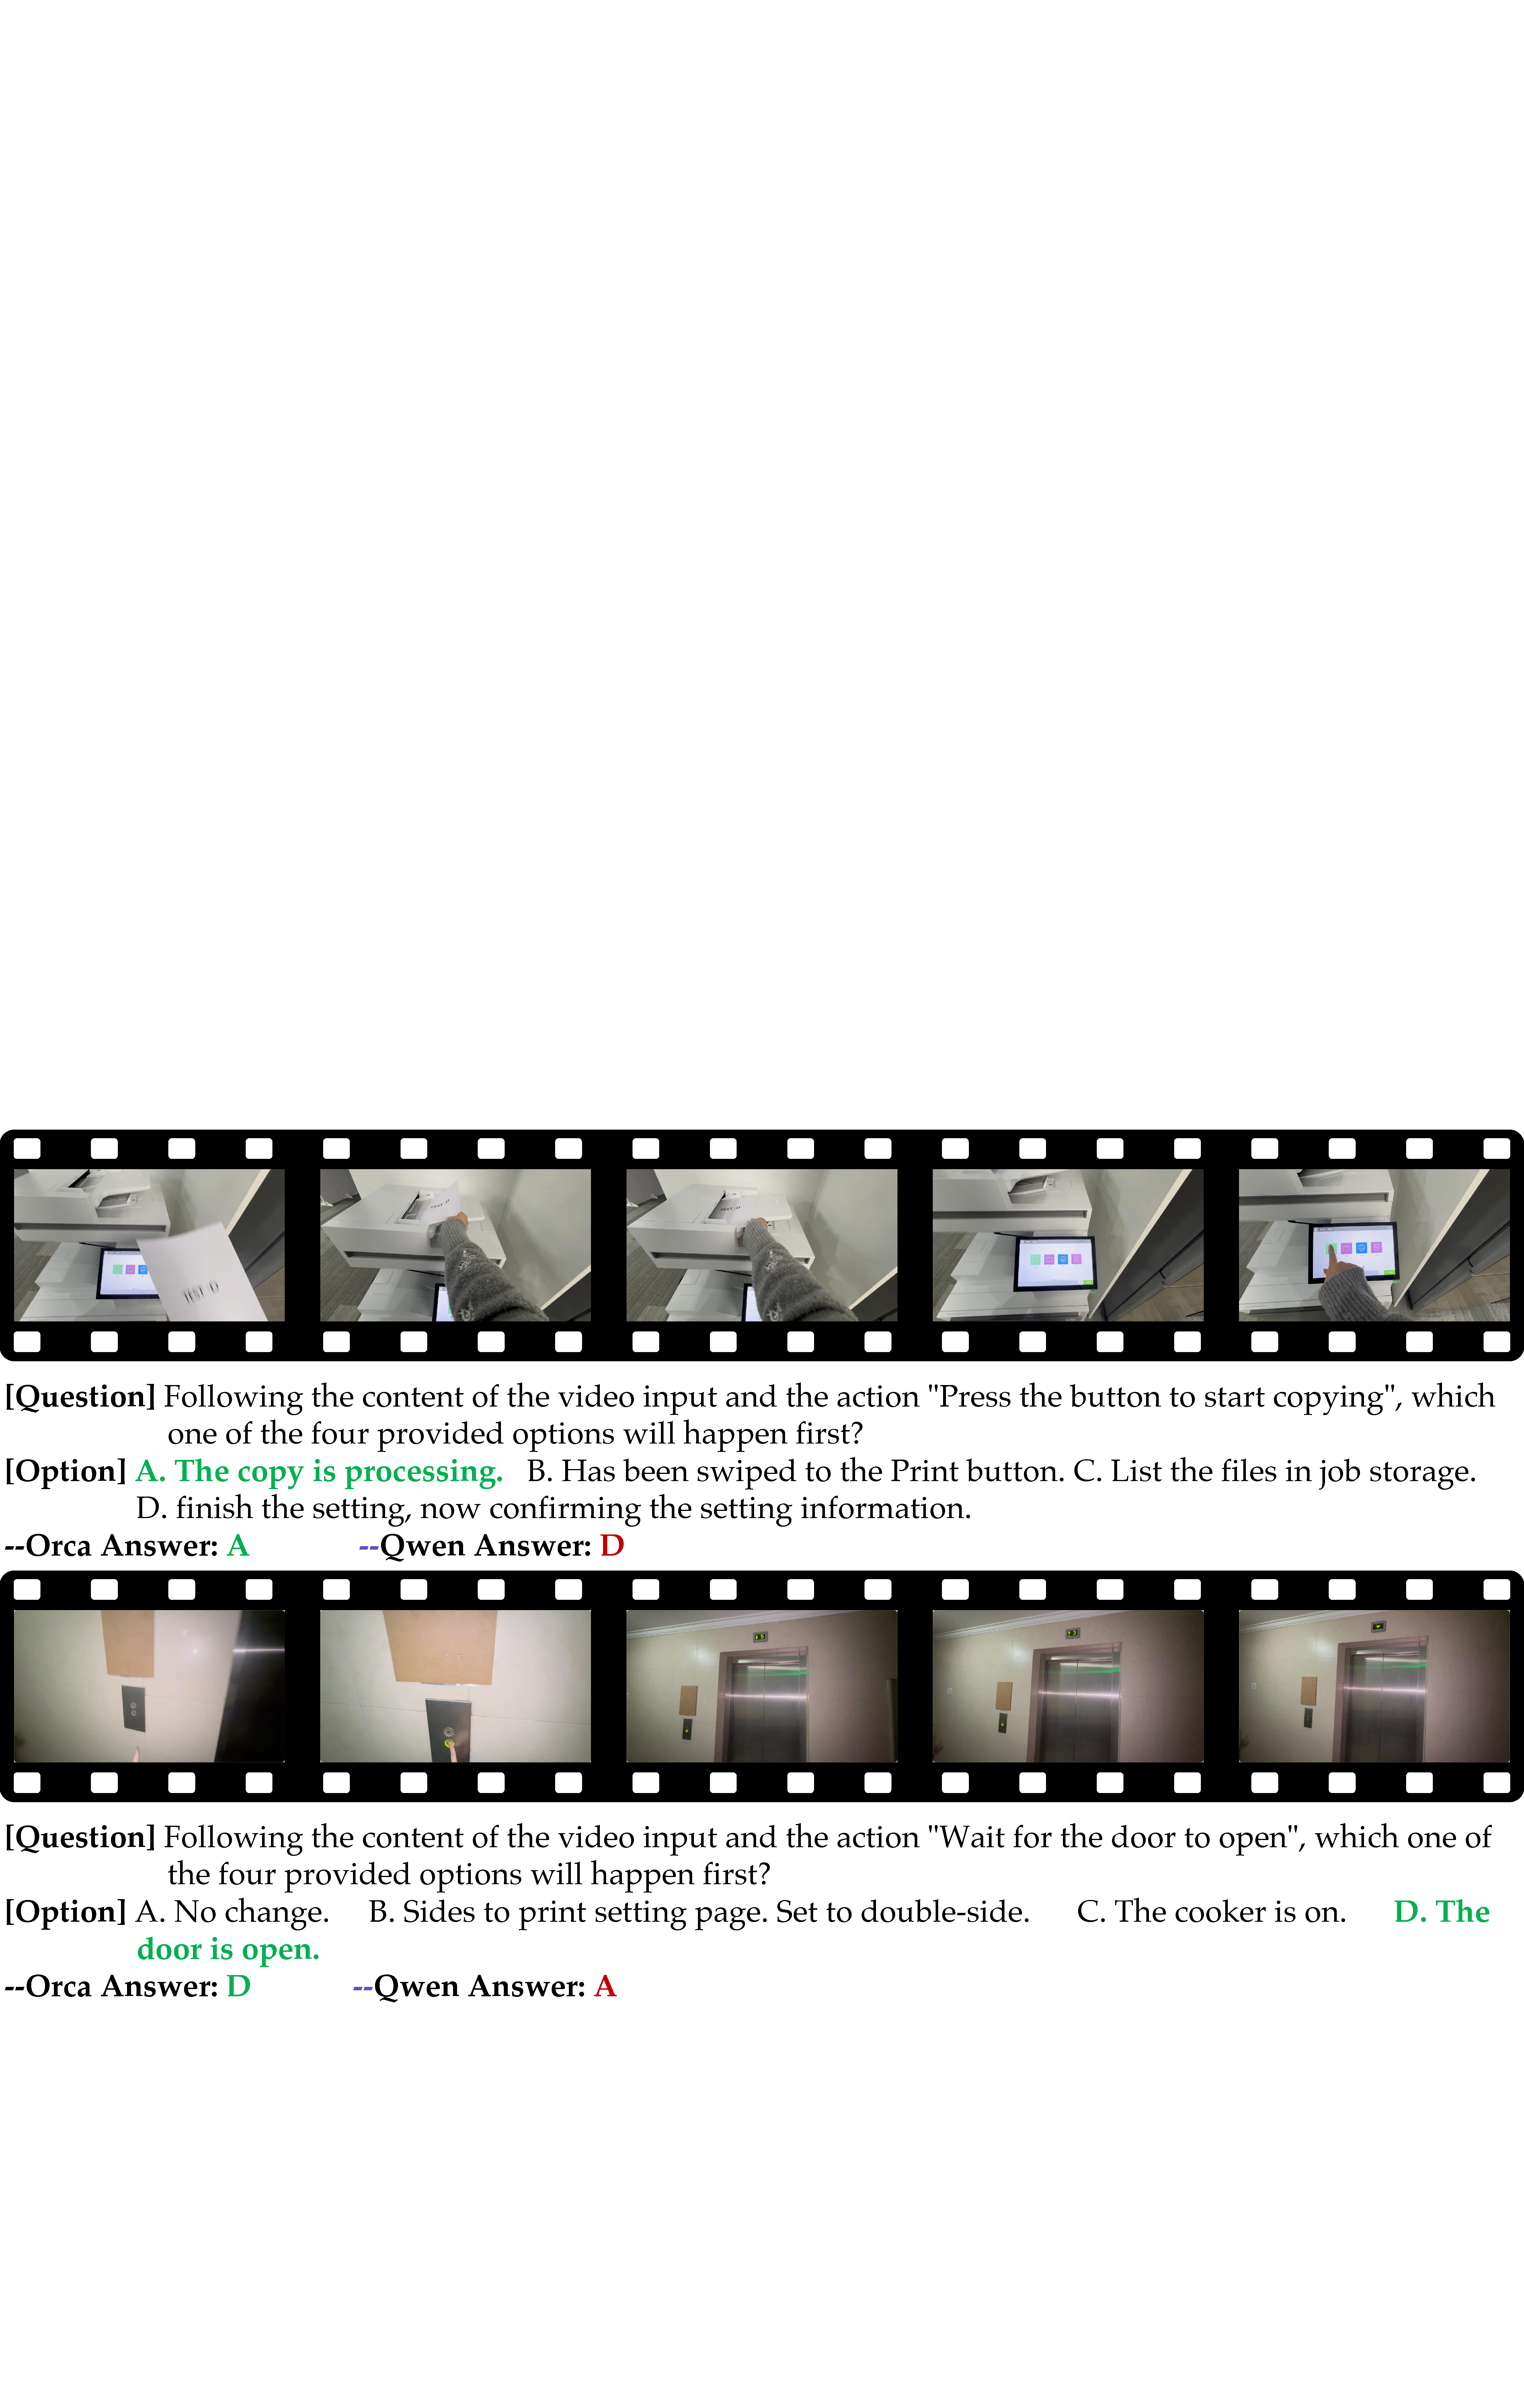
\includegraphics[width=0.75\linewidth]{figs/appendix/state-2.pdf}
  \caption{\textbf{More cross-benchmark examples of state transition.}}
  \label{fig:state-cross-bench2}
\end{figure}



\begin{figure}[!htbp]
    \centering
    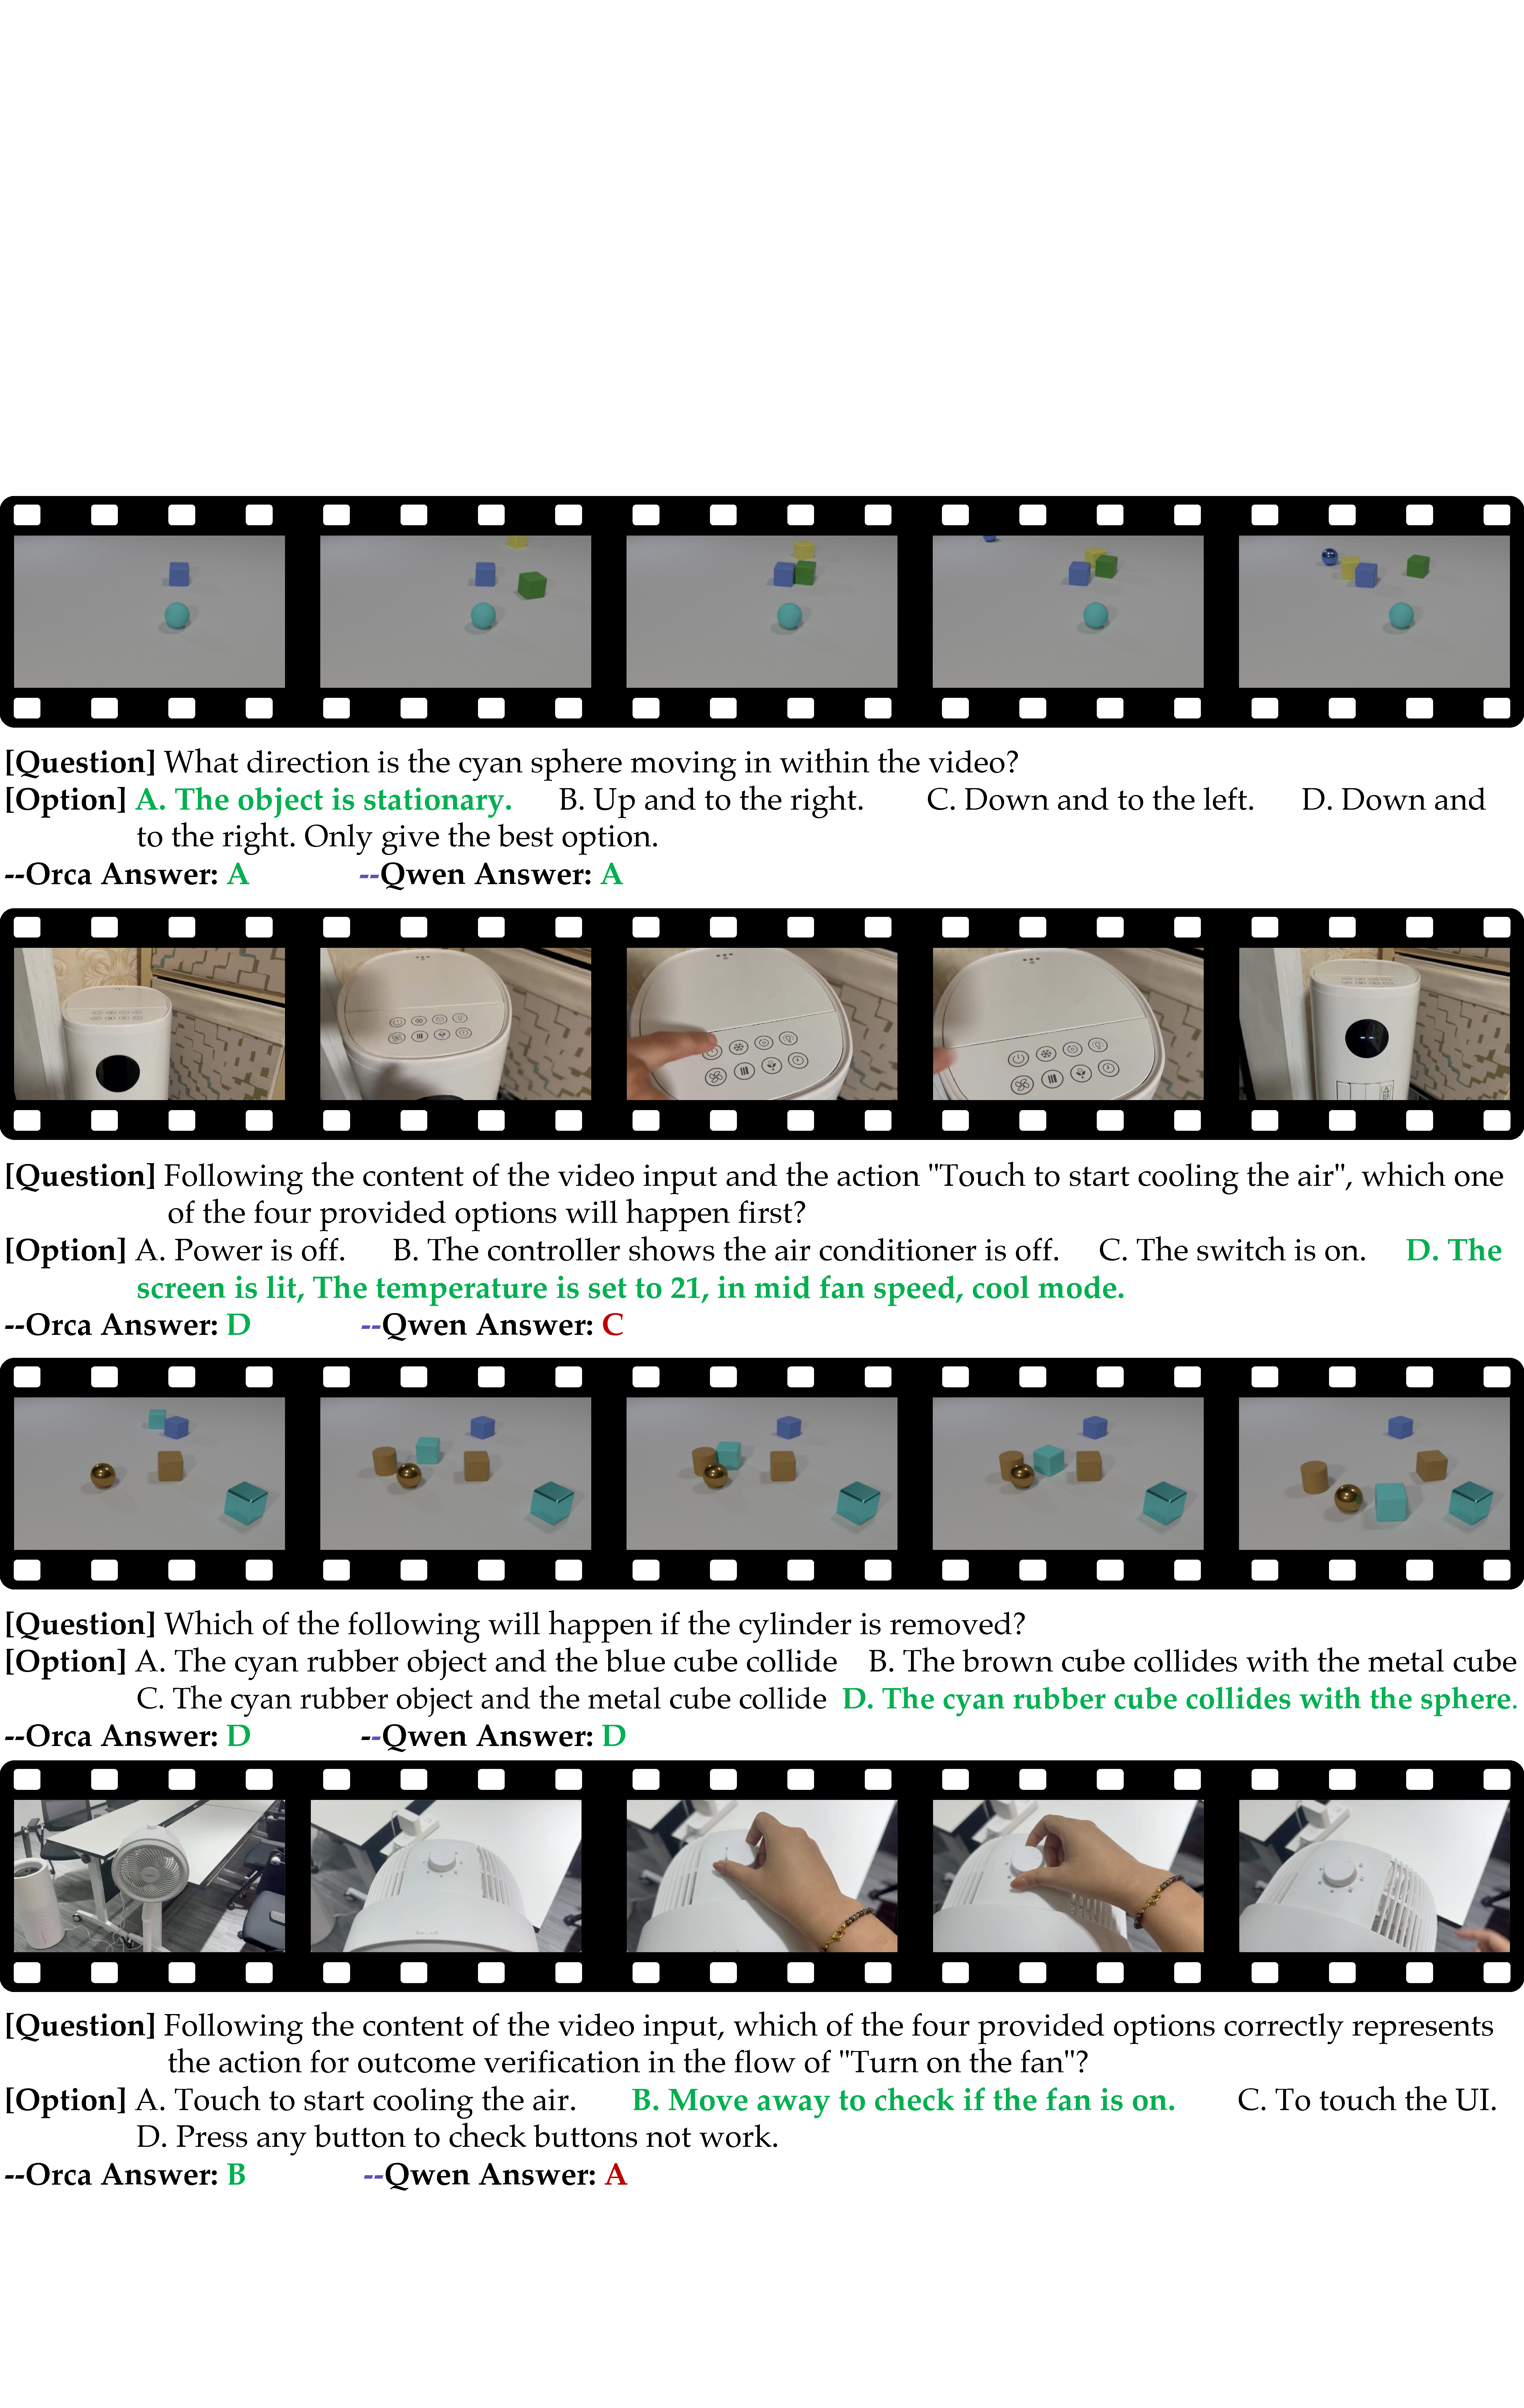
\includegraphics[width=0.75\linewidth]{figs/appendix/sense-1.pdf}
    \caption{\textbf{Cross-benchmark examples of commonsense reasoning.} The advantage of Orca is particularly pronounced in complex VQA scenarios that require reasoning beyond the visible scene and inferring hypothetical outcomes.}
    \label{fig:sense-cross-bench}
\end{figure}


\begin{figure}[!htbp]
    \centering
    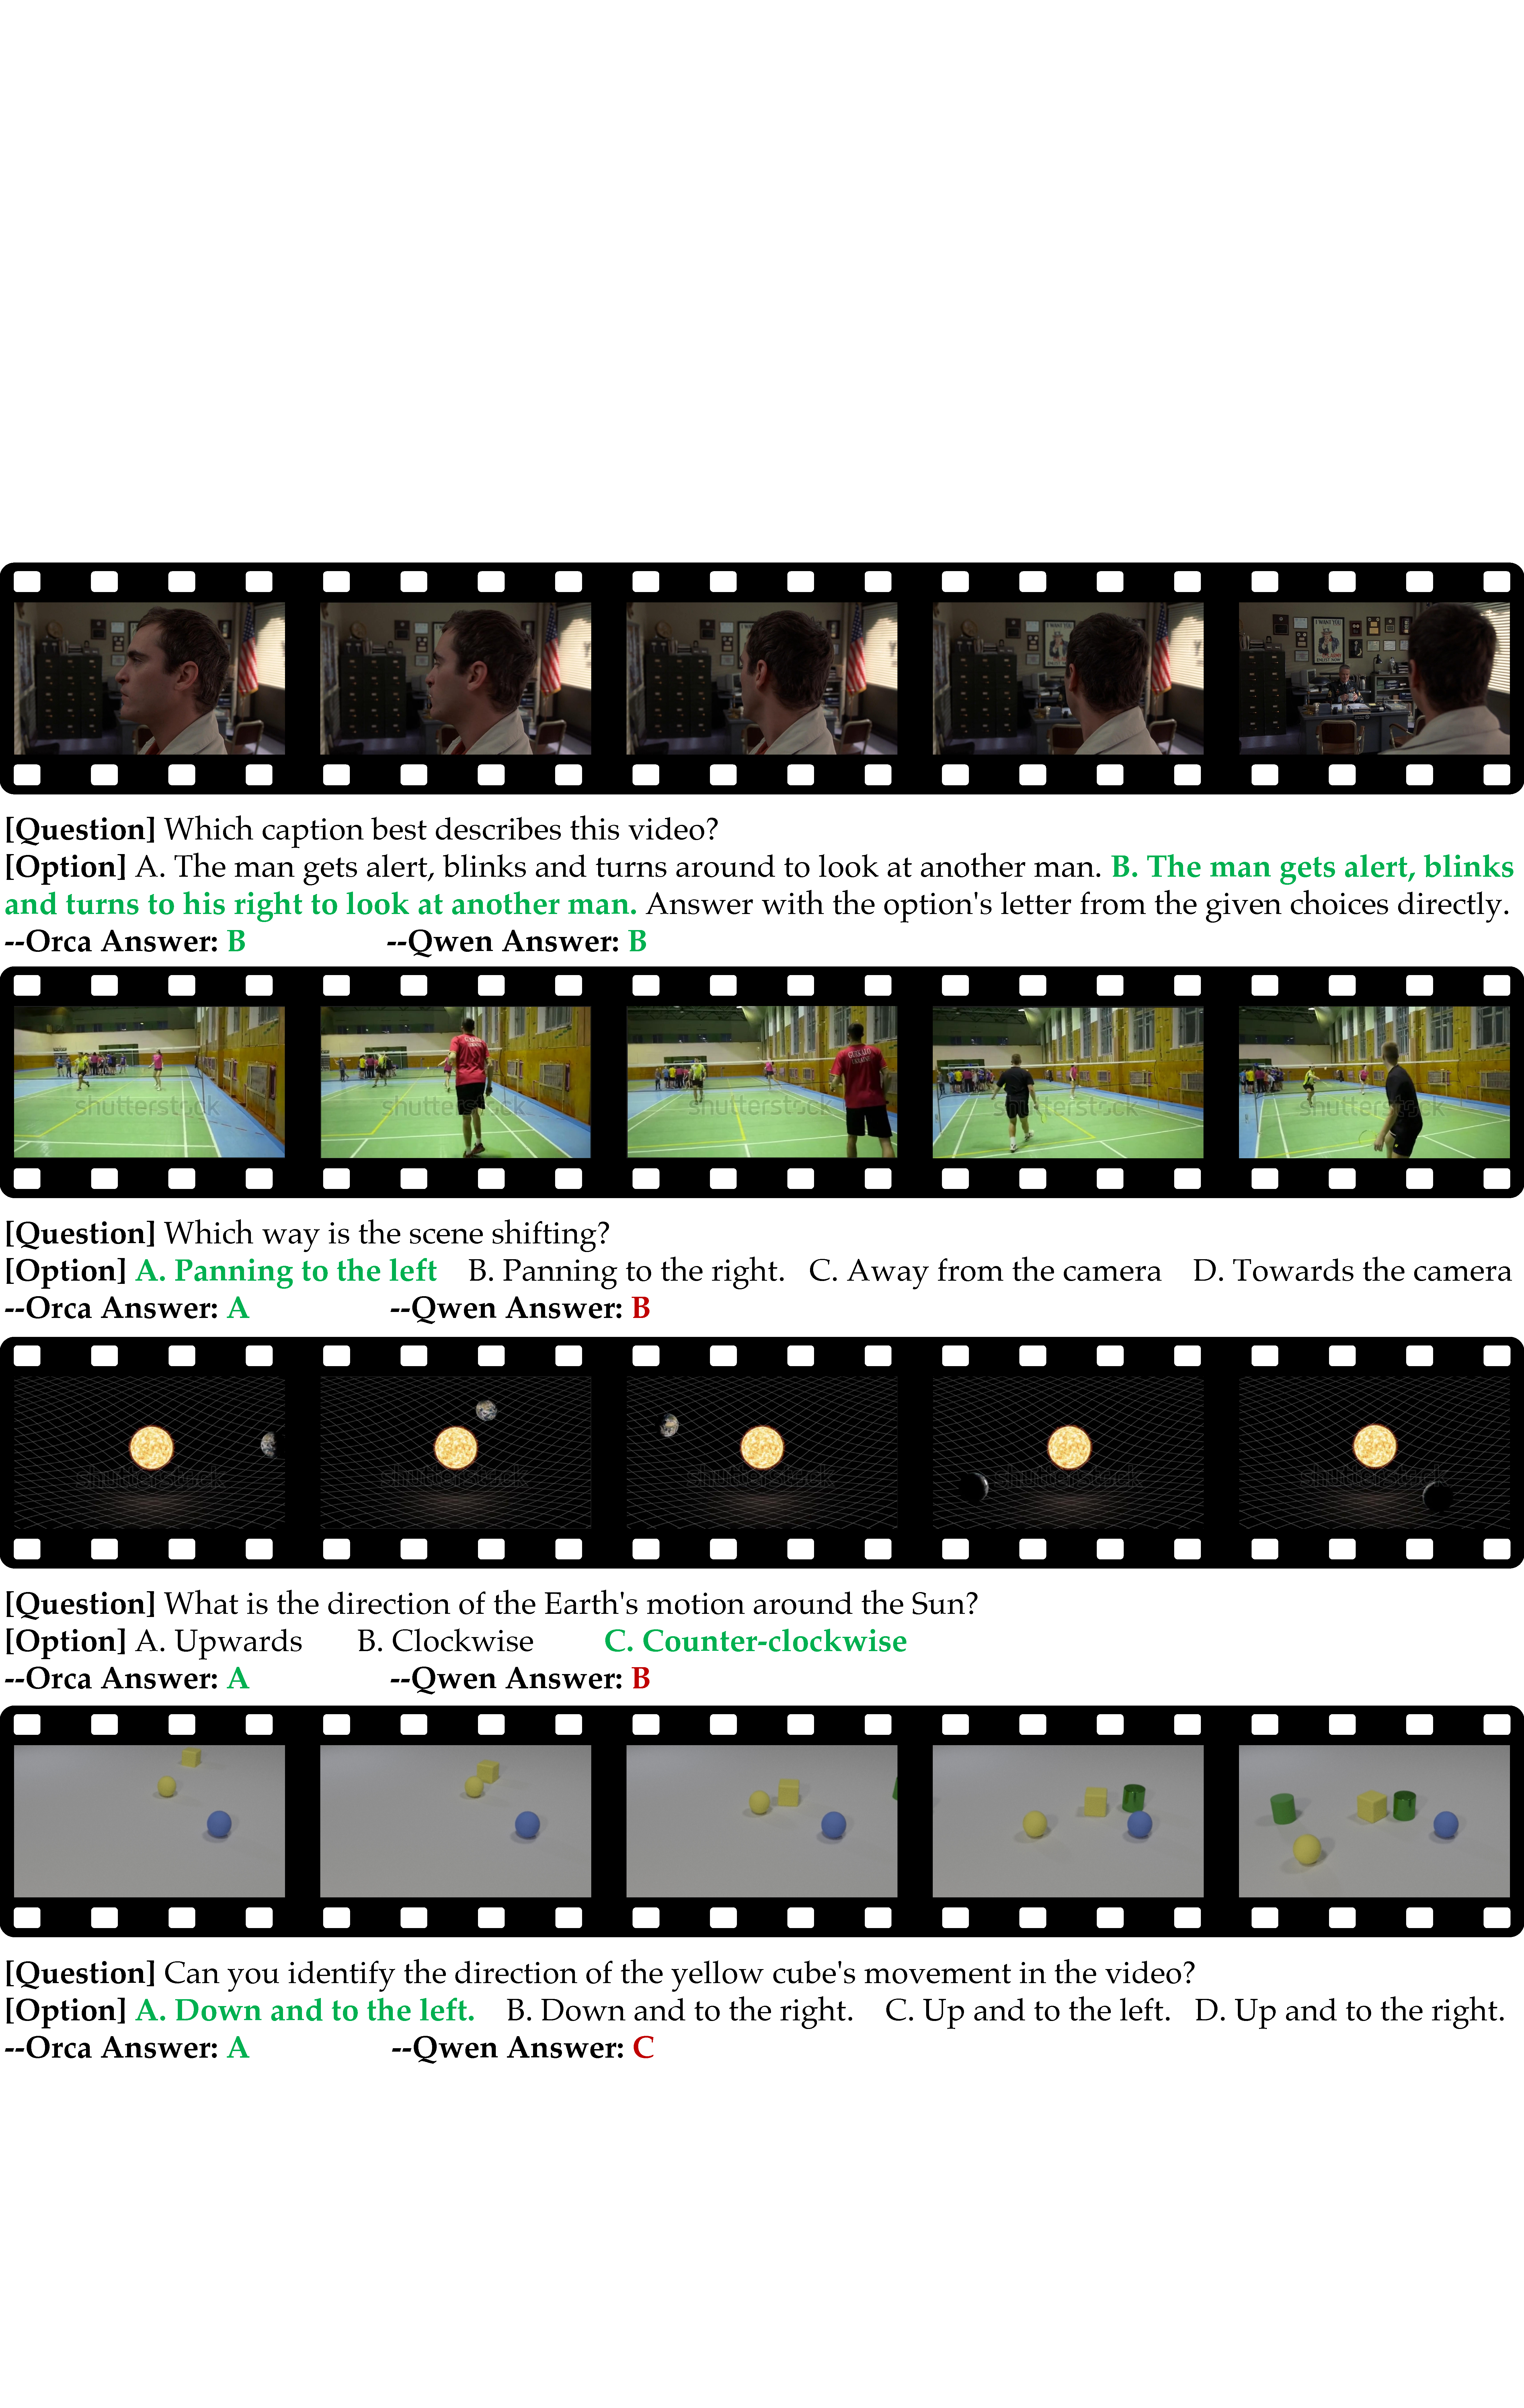
\includegraphics[width=0.95\linewidth]{figs/appendix/movement-1.pdf}
    \caption{\textbf{Cross-benchmark examples of dynamic motion.} The proposed unconscious learning paradigm enables Orca to naturally acquire temporal continuity and motion inertia, leading to stronger forward simulation capabilities for dynamic object behaviors.}
    \label{fig:move-cross-bench}
\end{figure}


\begin{figure}[!htbp]
    \centering
    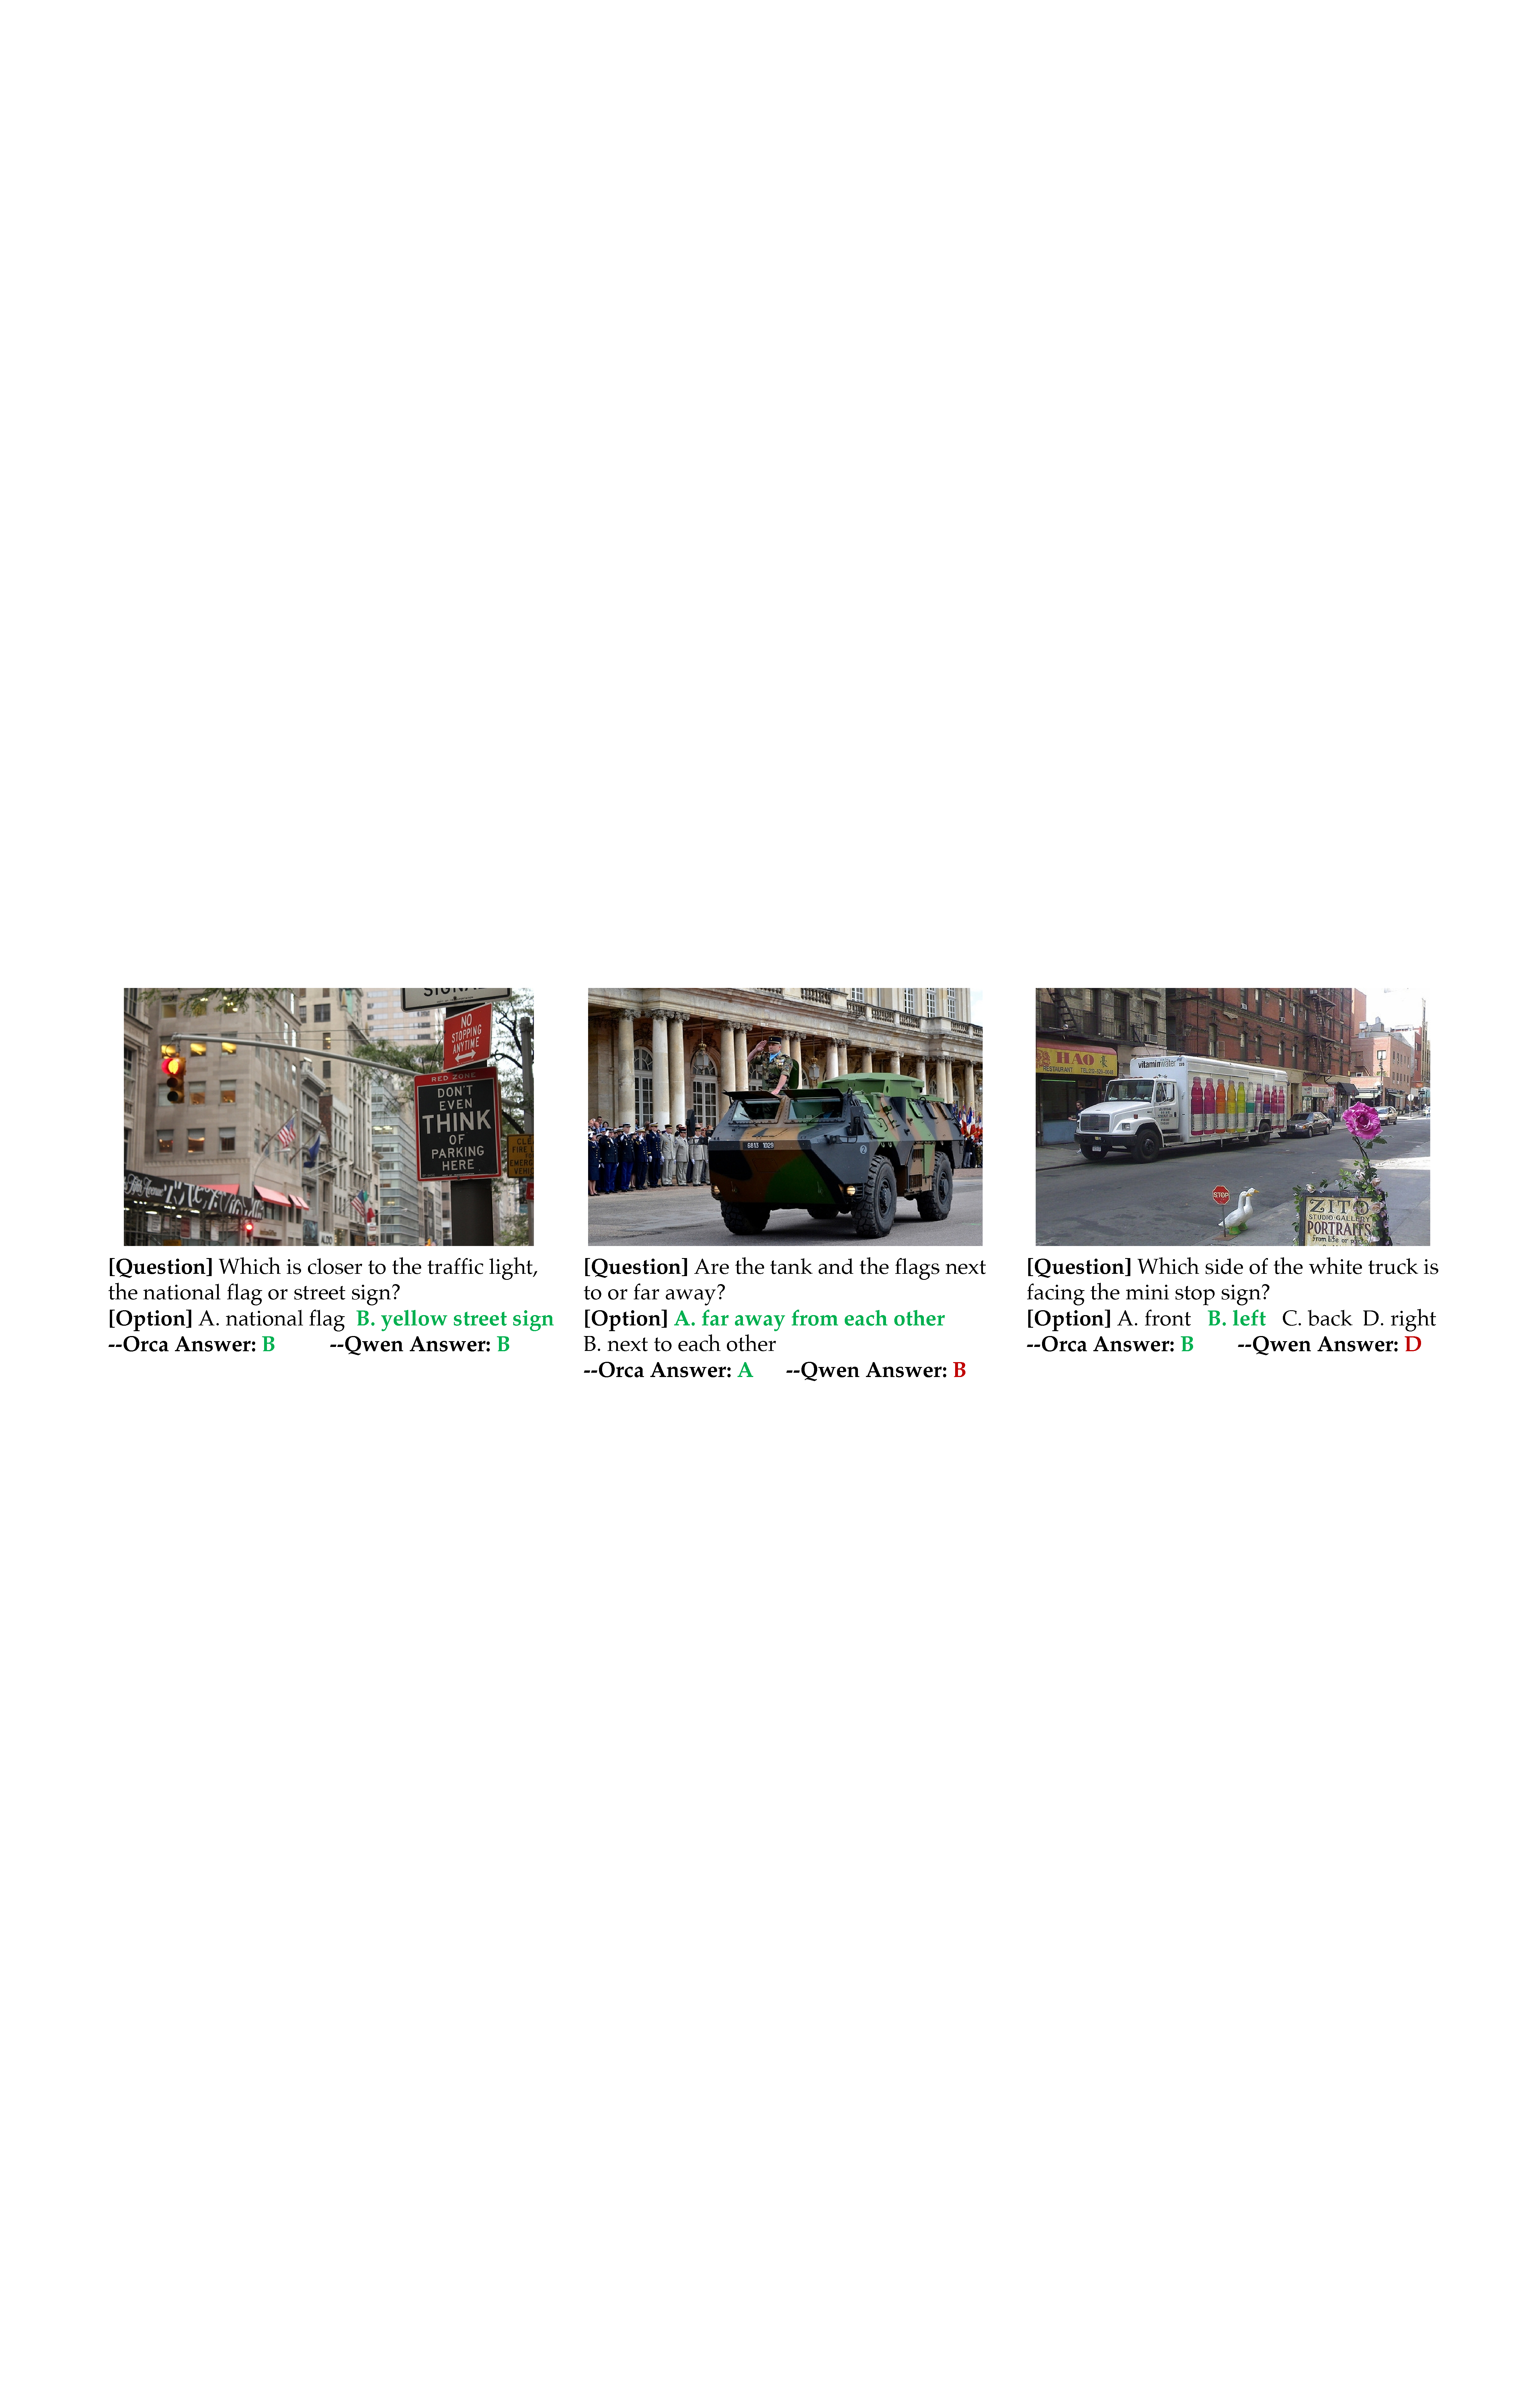
\includegraphics[width=1\linewidth]{figs/appendix/sp.pdf}
    \caption{\textbf{Cross-benchmark examples of spatial relations.} The results demonstrate strong robustness in scenarios involving complex occlusions and multi-object spatial reasoning.}
    \label{fig:spatial-cross-bench}
\end{figure}

